% Mathematical Optimization of Pacing Strategies in Competitive
% 200-Yard Freestyle Swimming
%
% Build:  cd paper && latexmk -pdf main.tex
% Bibliography is the repo's single source of truth:
% ../literature/references.bib (access-level notes included by the style).

\documentclass[11pt]{article}

\usepackage[margin=1.1in]{geometry}
\usepackage{amsmath,amssymb,amsthm}
\usepackage{graphicx}
\usepackage{booktabs}
\usepackage{microtype}
\usepackage[round]{natbib}
\usepackage{placeins}
\usepackage{xurl}
\usepackage[hidelinks]{hyperref}
\usepackage{underscore} % bib notes contain identifiers like beta_x

\graphicspath{{../figures/}{../figures/empirical/}}

\newtheorem{theorem}{Theorem}
\newtheorem{proposition}{Proposition}
\newtheorem{corollary}{Corollary}
\newtheorem{remark}{Remark}

\newcommand{\Erem}{E}
\newcommand{\dd}{\,\mathrm{d}}

\title{Mathematical Optimization of Pacing Strategies in Competitive
       200-Yard Freestyle Swimming}
\author{Om Joshi}
\date{Working draft --- \today}

\begin{document}
\maketitle

% Abstract — working-draft version. The empirical sentences will be finalized
% after the registered held-out comparison on the expanded dataset; nothing
% here claims results that do not yet exist.
\begin{abstract}
What pacing strategy minimizes 200-yard freestyle race time, and do
competitive swimmers use it? We formulate the four-lap race as a constrained
optimization problem over split velocities, with a cost function derived from
measured hydrodynamic drag, a two-parameter aerobic--anaerobic energy system,
and oxygen-uptake kinetics, and we prove two structural results. First, under
a fixed energy budget with velocity-only cost, even pacing is the unique
optimum --- a theorem, holding for every cost exponent $p>1$. Second, the
optimal pacing \emph{shape} is invariant to aerobic capacity, anaerobic
capacity, drag, and efficiency: those parameters set how fast the race is
swum, and provably not how it is divided. Because real 200-yard races are not
evenly paced, we formalize five competing fatigue mechanisms (constant
economy, oxygen kinetics, reserve-coupled cost, position-coupled cost, and a
fatigue-coupled velocity ceiling) that make three qualitatively distinct,
falsifiable predictions about split shape, and we test them against
anonymized official race results from male swimmers aged 15--18 under a
pre-registered analysis plan with a swimmer-grouped held-out test set. In the
pilot sample (80 races, one meet), every race is positively split,
sign-contradicting the reserve-coupled mechanism; the mean observed shape
lies within 0.3 percentage points of the front-loaded model family; and the
model ranking moves with the assumed dive-start credit across its
literature-anchored uncertainty band, making the start correction, rather
than the fatigue physics, the decisive open quantity. The registered
comparison on the expanded dataset, including fitted fatigue parameters and
the held-out evaluation, is reported in
Sections~\ref{sec:results-empirical}--\ref{sec:discussion}.
\end{abstract}

\section{Introduction}\label{sec:introduction}

The 200-yard freestyle occupies an awkward and interesting place in
competitive swimming: long enough that energy management decides the outcome,
short enough that the anaerobic reserve is a first-order quantity rather than
a correction. Coaches prescribe pacing for it with strong conviction and
little shared formalism. This paper asks the question underneath those
prescriptions: \emph{what pacing strategy minimizes 200-yard freestyle race
time under realistic energetic and fatigue constraints, and how closely do
successful real-world performances match it?}

The mathematical study of race pacing begins with
\citet{keller1973theory,keller1974optimal}, who derived optimal running
strategies from a bounded propulsive force, linear resistance, and a finite
energy reserve with constant aerobic resupply. The line he opened was
extended with richer, hydraulic energetics \citep{behncke1993mathematical},
fitted to world records from 50~m to 275~km \citep{woodside1991optimal},
augmented with explicit fatigue states \citep{mathis1989fatigue}, and, in the
modern optimal-control treatment of \citet{aftalionbonnans2014}, shown to
favor deliberate velocity variation once anaerobic energy can be partially
re-created during deceleration. Swimming has been touched by this line
exactly once at the level of formal optimal control: \citet{maronski1996minimum}
derived a minimum-time swim profile --- glide, cruise, terminal kick --- from
a two-equation model. What the swimming literature has in abundance instead
is careful \emph{description}: elite 200-m freestyle finalists swim a fast
first lap followed by a nearly flat back half \citep{robertson2009analysis},
fast-start profiles dominate at every level, and pacing skill discriminates
finalists from non-qualifiers. Description and optimization have largely not
met, and where models exist they are typically fitted to records rather than
tested against the split sheets of ordinary competitive races.

This paper tries to make them meet, for one event, one course, and one
population: the 200-yard short-course freestyle swum by male competitive
swimmers aged 15--18. The contributions are four.

\paragraph{A theorem where a simulation is expected.} Under a fixed energy
budget and a velocity-only cost function, the four-split problem is a convex
program whose unique optimum is exactly even pacing, for every cost exponent
$p>1$ and every parameter choice (Section~\ref{sec:theorems}). Even pacing is
therefore not a finding about our parameters but a structural property of
budget-constrained racing, and every departure of real races from even pacing
is evidence about mechanisms \emph{outside} that structure.

\paragraph{Shape--engine separation.} With position-coupled economy decay the
optimal split allocation has a closed form, $t_i \propto w_i^{1/p}$, whose
striking consequence is that aerobic capacity, anaerobic capacity, drag and
efficiency have \emph{no effect at all} on the optimal shape
(Section~\ref{sec:theorems}). A swimmer with a bigger engine should swim the
same shape, faster. The popular intuition that stronger athletes have earned
a faster opening lap has no support in this model class.

\paragraph{Competing mechanisms as competing predictions.} We formalize five
fatigue mechanisms --- none of them exotic, all of them present somewhere in
the running literature --- and show they collapse onto three qualitatively
distinct split shapes: exactly even, strongly negative, and two
distinguishable kinds of positive (Section~\ref{sec:competing}). This turns
``which fatigue story is true'' into a sign-and-shape question that a few
dozen official split sheets can already inform.

\paragraph{Pre-registered confrontation with real races.} We built a
verified data pipeline for official age-group race results (anonymized at
ingest; swimmer-grouped train/test split; analysis plan and amendment log
frozen before any fitting) and report the confrontation honestly, including
the finding that currently dominates all others: the comparison is decided
less by fatigue physics than by the dive-start credit, whose
literature-anchored uncertainty band spans the distance between the
competing models (Sections~\ref{sec:data}--\ref{sec:results-empirical}).

Two boundaries are drawn deliberately. We optimize a clock, not a field:
tactical racing, drafting and psychology are outside the model. And we treat
within-lap velocity as constant, which excludes by assumption the
oscillation mechanisms of \citet{aftalionbonnans2014}; split-level data
cannot resolve within-lap dynamics in either direction, so this is a stated
limitation rather than a hidden one (Section~\ref{sec:limitations}).

\section{The Model}\label{sec:model}

\subsection{Race, control, objective}

A 200-yard short-course race covers $L = 182.88$~m in a 25-yard pool,
recorded as four cumulative 50-yard splits. The control is the velocity
profile; in the discrete model the swimmer chooses one velocity per 50,
$v = (v_1,\dots,v_4)$, $v_i \in [v_{\min}, v_{\max}]$, and the objective is
the race time
\begin{equation}
  T(v) \;=\; \sum_{i=1}^{4} \frac{d}{v_i},
  \qquad d = L/4 = 45.72~\text{m}.
  \label{eq:objective}
\end{equation}

\subsection{Cost of speed, from drag}

Steady swimming against hydrodynamic drag $F_D = \tfrac12 \rho C_D A v^2$
requires mechanical power $P = F_D v = K_d v^3$ with
$K_d = \tfrac12 \rho C_D A$. Propulsion converts metabolic power to useful
thrust with propelling efficiency $\eta_p$ and gross efficiency $\eta_g$, so
the metabolic cost rate of swimming at velocity $v$ is
\begin{equation}
  C(v) \;=\; \phi\,\frac{K_d}{\eta_p \eta_g}\, v^{3}
        \;=\; k\, v^{p}, \qquad p = 3 .
  \label{eq:cost}
\end{equation}
The drag block uses measured values ($C_D = 0.30$, $A = 0.230$~m$^2$,
active-drag literature), giving $K_d = 34.4$ inside the independently
measured 22--38~kg/m band. Two honesty notes attach to
Eq.~\eqref{eq:cost}. First, published gross efficiencies disagree by a factor
of $3$--$4$ for definitional reasons, so $k$ is \emph{not identifiable from
the literature} and every absolute energy in this paper is model-internal.
Second, $\phi \in (0,1]$ is a \emph{course economy factor}, the model's one
openly calibrated scalar: it names the per-metre discount of racing in a
short-course pool, where turn sections occupy roughly half of total race time
and wall push-offs and underwater kicking move the swimmer 20--30\% faster
than surface swimming \citep{cuencafernandez2022turn, born2022imsections,
veiga2022underwater}. The measured turn literature brackets the expected
discount at roughly $\phi \in [0.80, 0.95]$; the calibrated values across
model variants span 0.77--1.00.

\subsection{Energy system}

The engine is a two-parameter critical-power structure: an aerobic supply
ceiling $R$ and a finite anaerobic reserve $E_0$, with optional oxygen-uptake
kinetics of time constant $\tau$. With distance $x$ as independent variable
and states $t(x)$ (elapsed time) and $\Erem(x)$ (remaining reserve),
\begin{equation}
  \frac{\dd t}{\dd x} = \frac{1}{v(x)}, \qquad
  \frac{\dd \Erem}{\dd x} = \frac{R\big(t(x)\big) - C\big(v(x)\big)}{v(x)},
  \qquad
  R(t) = R\big(1 - e^{-t/\tau}\big),
  \label{eq:dynamics}
\end{equation}
with $t(0)=0$, $\Erem(0)=E_0$, the path constraint $\Erem(x) \ge 0$ (a
swimmer cannot borrow energy), and free terminal reserve. Setting $\tau = 0$
recovers instantaneous aerobic supply. The reference calibration
($R = 1250$~W, $E_0 = 50.3$~kJ at the model-internal $k$) reproduces a
1:40.0 optimum for the target population; this is a calibration to a target
time, not a physiological measurement, and the identifiability analysis in
the repository documents which parameters race data can and cannot pin down.
The engine's aerobic--anaerobic proportions are independently checked against
the swimming critical-speed literature: the model's dimensionless ratio of
critical speed to 200-m race speed is 0.893 against a measured 0.898 for
trained male adolescents \citep{nikitakis2019cs}, with an implied anaerobic
distance capacity of 19.5~m inside the measured 14--31~m band
\citep{zacca2010critical, machado2009cv}.

\subsection{Raced space and recorded space}

The model describes free swimming from a moving start; a recorded race
includes a dive, which makes recorded lap~1 \emph{faster} than swimming it at
race pace. Measured elite 15-m start times imply a dive value of
1.7--3.0~s at elite pace, and the same measurements imply
$S(v) \approx 15/v - t_{15}$, i.e.\ a larger credit at slower field paces. A
course-level start credit $S$ (default 1.80~s, elite-anchored, Category~B
provenance) maps between the two spaces: model~$\to$~recorded subtracts $S$
from lap~1; data~$\to$~raced adds it back. Exactly one transform is applied
per comparison. Because $S$ is a constant time credit it cannot change which
velocity profile is optimal, so it never enters the optimizer --- but it
turns out to sit directly on the model comparison, a point
Section~\ref{sec:results-empirical} returns to at length.

%% Section stub: filled by its own commit per ATOMIC_COMMIT_ROADMAP.md
\section{Structural Results}\label{sec:theorems}
[Pending.]

%% Section stub: filled by its own commit per ATOMIC_COMMIT_ROADMAP.md
\section{Competing Fatigue Models}\label{sec:competing}
[Pending.]

%% Section stub: filled by its own commit per ATOMIC_COMMIT_ROADMAP.md
\section{Data}\label{sec:data}
[Pending.]

\section{Validation Methods}\label{sec:methods}

The analysis plan was written on 29~August~2026, when zero races were in
hand, and is kept in the repository with an amendment log. Everything in
this section was fixed before any parameter was fitted to any race. The
plan's function is to make the empirical section falsifiable in advance:
what is measured, what counts as a win, what is fitted, and what is done
about the dive start were all decided when the data could not yet influence
the decision.

\subsection{Primary metric}

For each race with cumulative splits $S_1<S_2<S_3<S_4=T$ we form lap times
$s_i=S_i-S_{i-1}$ and the free-swimming-equivalent shares
\begin{equation}
  P_i \;=\; \frac{s_i + \delta_{i1}\,c}{T + c}, \qquad i=1,\dots,4,
  \label{eq:shares}
\end{equation}
where $c$ is the dive-start credit added back to lap~1
(Section~\ref{sec:start}). The model predicts raced-space fractions
$P_i^\ast$, and the per-race primary metric is
$\mathrm{RMSE}=\big[\tfrac14\sum_i (P_i-P_i^\ast)^2\big]^{1/2}$, reported
in percentage points and averaged over races. The metric is scale-free, so a
1:37 swimmer and a 2:30 swimmer contribute comparably. Because the $P_i$ sum
to one, only three residuals are free; RMSE over four terms remains a valid
comparison statistic since every model is scored identically, but it is
never treated as having four independent components. Secondary metrics are
the mean absolute error, the per-lap signed error (which is what actually
separates M3 from M4), and the pre-registered discriminator: the lap
$1\!\to\!2$ drop against the lap $3\!\to\!4$ drop. Race-time error is
reported but never used for selection, because race time depends on
parameters the shape cannot identify (Theorem~\ref{thm:shape}). Likelihood
criteria such as AIC are not used: the models are deterministic and carry no
error model, and inventing one for the convenience of a statistic would be a
modelling choice made backwards.

\subsection{What counts as a win}

A model \emph{wins on shape} if its predicted sign of $P_4-P_1$ matches the
observed mean's and no other model's does; M0 and M1 are shape-identical and
count once. A model \emph{wins on accuracy} if its held-out mean RMSE is
lower than every other model's by more than the 95\% bootstrap confidence
half-width of that difference. If neither criterion separates the models,
the registered conclusion is that the data do not distinguish them, and
that is reported as the result.

\subsection{Split, fitting, and the leakage guard}

Races are split into training and test sets \emph{by swimmer}, never by race:
repeated races from one swimmer share technique, start quality and habitual
pacing, so a race-level split would score models partly on how well they
memorized individuals. Swimmers are assigned whole to one side until the
test side holds at least a quarter of the races, with a seed (20260829)
fixed in the plan. On pilot-v0.2 this gives 256 training races by 188
swimmers and 89 held-out races by 60 swimmers. Fitting code can obtain data
only through a function that withholds the test rows, and a structural guard
raises an exception if any frame containing a held-out swimmer reaches an
objective; the guard is unit-tested. The test set is opened once, by one
script, which records the time it did so.

Exactly one parameter per model is fitted to shape: $\beta_E$ for M2,
$\beta_x$ for M3, $\gamma$ for M4; M0 and M1 have none. Nothing else is
fitted to pacing data. By Theorem~\ref{thm:shape} the engine parameters
($E_0$, $R$, $\tau$), the drag block and the efficiencies do not enter the
optimal shape, so fitting them to splits would produce numbers that are
pure noise, and reporting those as physiology would be the worst error
available to this project. Each fit minimizes the mean training RMSE over
its parameter: for M3 the shape is closed-form and a bounded scalar search
is exact; for M2 and M4 every objective evaluation is an inner
optimal-control solve, so a coarse grid brackets the minimum and a bounded
Brent refinement follows, with the evaluation budget recorded. One free
parameter each makes the comparison fair without a complexity penalty.

\subsection{The dive start}\label{sec:start}

The model describes free swimming; recorded lap~1 contains a dive. Because
the start and both positive-split couplings push lap~1 the same way, an
uncorrected fit would absorb the dive into the fatigue parameter and
overstate it. The plan therefore (i) adds a credit $c$ to lap~1 before
computing shares, with $c=1.80$~s anchored to measured elite 15~m start
times \citep{tor2014characteristics,rudnik2023kinematic}; (ii) reports every
headline result across a sensitivity band, originally 1.2--2.4~s and
widened by two logged amendments to 1.2--3.4~s once those same start times
were converted to this field's slower race pace
($c \approx 15/\bar v - t_{15} \approx 3.1$--$3.4$~s); and (iii) rules that
if the model ranking changes anywhere inside the band, the conclusion is
that the data cannot distinguish the models given start uncertainty. A
third amendment, logged on 1~September~2026, corrected a sign error in the
implementation of item~(i): the credit had been subtracted from observed
lap~1 as well as from the model's, double-counting it. The metric definition
did not change; the code was made to match it, and every pilot output was
regenerated. All three amendments preceded any calibration and any use of
the test set, and appear in the plan's amendment log rather than as silent
edits.

\subsection{Deviation and performance}

The primary hypothesis is that swimmers whose pacing lies closer to the
predicted optimum perform better relative to expectation. For race $j$ of
swimmer $i$ we compute the deviation $D_{ij}$, the RMSE of the race's shares
from the best-supported model's fitted optimum, and the relative improvement
$I_{ij}=(T^{\mathrm{PB}}_{ij}-T_{ij})/T^{\mathrm{PB}}_{ij}$, where
$T^{\mathrm{PB}}_{ij}$ is the swimmer's best time \emph{before} that race; a
later best would leak the outcome into the predictor. The registered model is
a mixed-effects regression with a random intercept per swimmer,
$I_{ij}=b_0+b_1 D_{ij}+b_2 D_{ij}^2+u_i+e_{ij}$, quadratic because the
theory predicts a quadratic penalty near the optimum
(Section~\ref{sec:results-theory}), with a pre-registered fallback to
ordinary least squares with swimmer-clustered standard errors if the
random-effect variance is not identifiable at the achieved sample size.
Confidence intervals for every held-out quantity are percentile bootstrap
intervals that resample swimmers, not races (10{,}000 draws, one resample
applied to all models so that differences are computed on matched draws).

\subsection{Power, stated in advance}

The theoretical effect is small: a 5\% opening error costs about
0.09~s in 100~s, while meet-to-meet variation in a swimmer's 200 free is of
order 1\%. The plan states that even 200--300 races may be underpowered for
the deviation--performance relationship and that a null there will be
reported as a null. The model-comparison question is better powered, because
the shape differences between M2, M3 and M4 are large relative to the
race-to-race noise in shares.

\subsection{Exploratory versus registered}

The 80-race first pilot was used to exercise the fitting machinery and to
quantify the start-credit confound; those fits are labelled exploratory in
the repository and are not the calibration. The registered calibration was
run on the training side of the frozen pilot-v0.2 dataset after the freeze
(with one inner-solver fix, described in
Section~\ref{sec:results-empirical}, made and logged before the test set
was opened); the held-out evaluation was then run once on its test side. All code, the plan, its amendments, the dataset
register with source digests, and a continuous-integration test suite are in
the project repository. The anonymized race table itself is not published,
because ages, teams and exact times at named meets would re-identify
minors; the chain from official result sheet to every number in this paper
can nonetheless be re-executed by anyone holding those public sheets, whose
digests are recorded.

\section{Theoretical Results}\label{sec:results-theory}

This section reports what the model says before any race is consulted. All
numbers are produced by the repository's \texttt{run\_all} script from the
parameter registry; the reference swimmer is calibrated so that the optimal
200-yard time is exactly 100.0~s (1:40.0), which makes penalties readable as
seconds lost per 100~s of racing.

\subsection{The optimum and the cost of missing it}

Under the pure budget (M0) the optimum is four laps of 25.000~s, and the
closed form, the split-space SQP solve and the direct ODE integration agree
on it to $10^{-11}$~s, as Theorem~\ref{thm:even} requires. The interesting
quantity is not the optimum but the penalty for missing it, because the
penalty is what a coach would act on. Figure~\ref{fig:penalty} plots the
race time when the opening lap is forced to a fixed error and the remaining
three laps are re-optimized around it. The penalty is quadratic near the
optimum and small: a 2\% opening error costs 0.015~s, 5\% costs 0.09~s, and
10\% costs 0.36~s (too fast) or 0.39~s (too slow). Named strategies at the
same energy budget tell the same story (Figure~\ref{fig:strategies}): a
smooth ramp spanning 1.5 points from first lap to last, in either
direction, costs 0.055~s; the ``aggressive opening'' profile, 7.4\% fast on
lap~1, costs 0.27~s; a ``very aggressive'' 13.0\% opening costs 0.94~s; a
conservative 6.4\% slow opening costs 0.18~s. The corrected elite 200-m finalist profile of
\citet{robertson2009analysis} costs 0.009~s against the even optimum, and
the mean corrected profile of our own 80-race first pilot costs 0.075~s. A
Monte Carlo over the physiological block (240 draws with $R$, $E_0$, $C_D$,
$A$, $\eta_p$, $\eta_g$ perturbed log-normally at 10\% coefficient of
variation; Figure~\ref{fig:robust}) leaves this ordering intact in every
draw, with the very-aggressive penalty spanning 0.83--1.06~s and the smooth
ramps 0.049--0.063~s across the 5th--95th percentiles. The ranking of
pacing errors is therefore robust to parameter ignorance of the size we
actually have; the magnitude is robust to within about 15\%.

\begin{figure}[htbp]
\centering
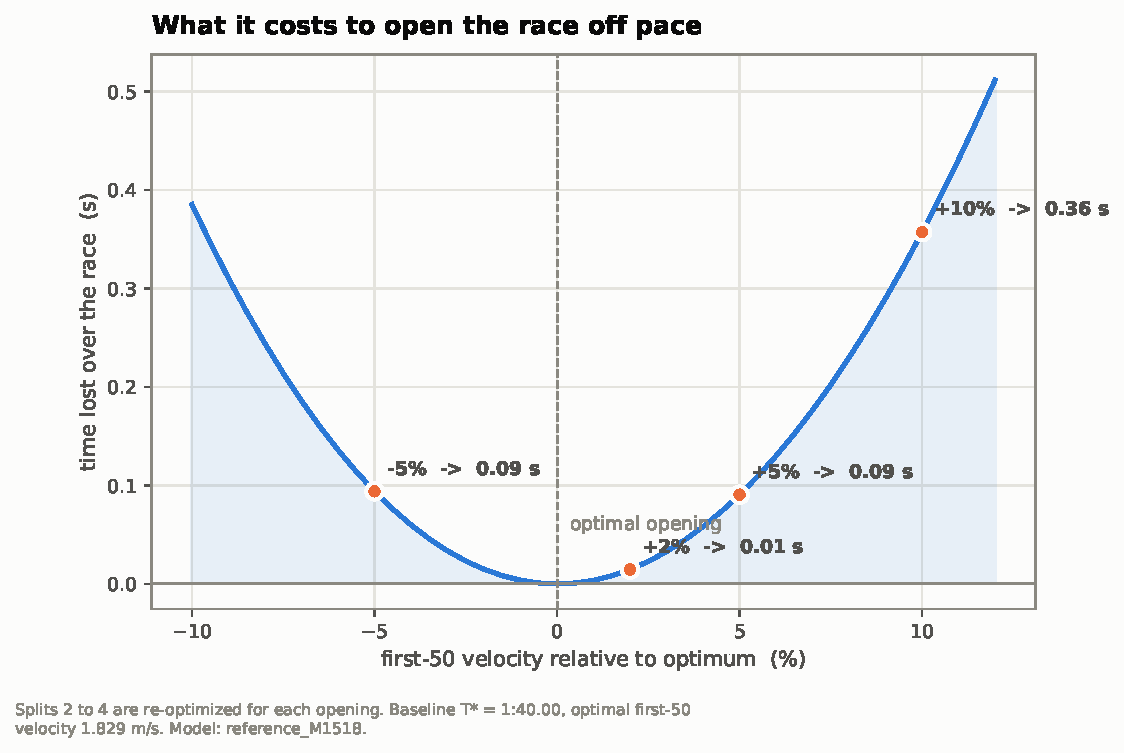
\includegraphics[width=0.62\linewidth]{fig05_opening_penalty}
\caption{Race-time penalty for a forced opening-lap error, remaining laps
re-optimized (reference swimmer, M0). The penalty is quadratic near the
optimum; a 5\% opening error costs about 0.09~s of a 100~s race.}
\label{fig:penalty}
\end{figure}

\begin{figure}[htbp]
\centering
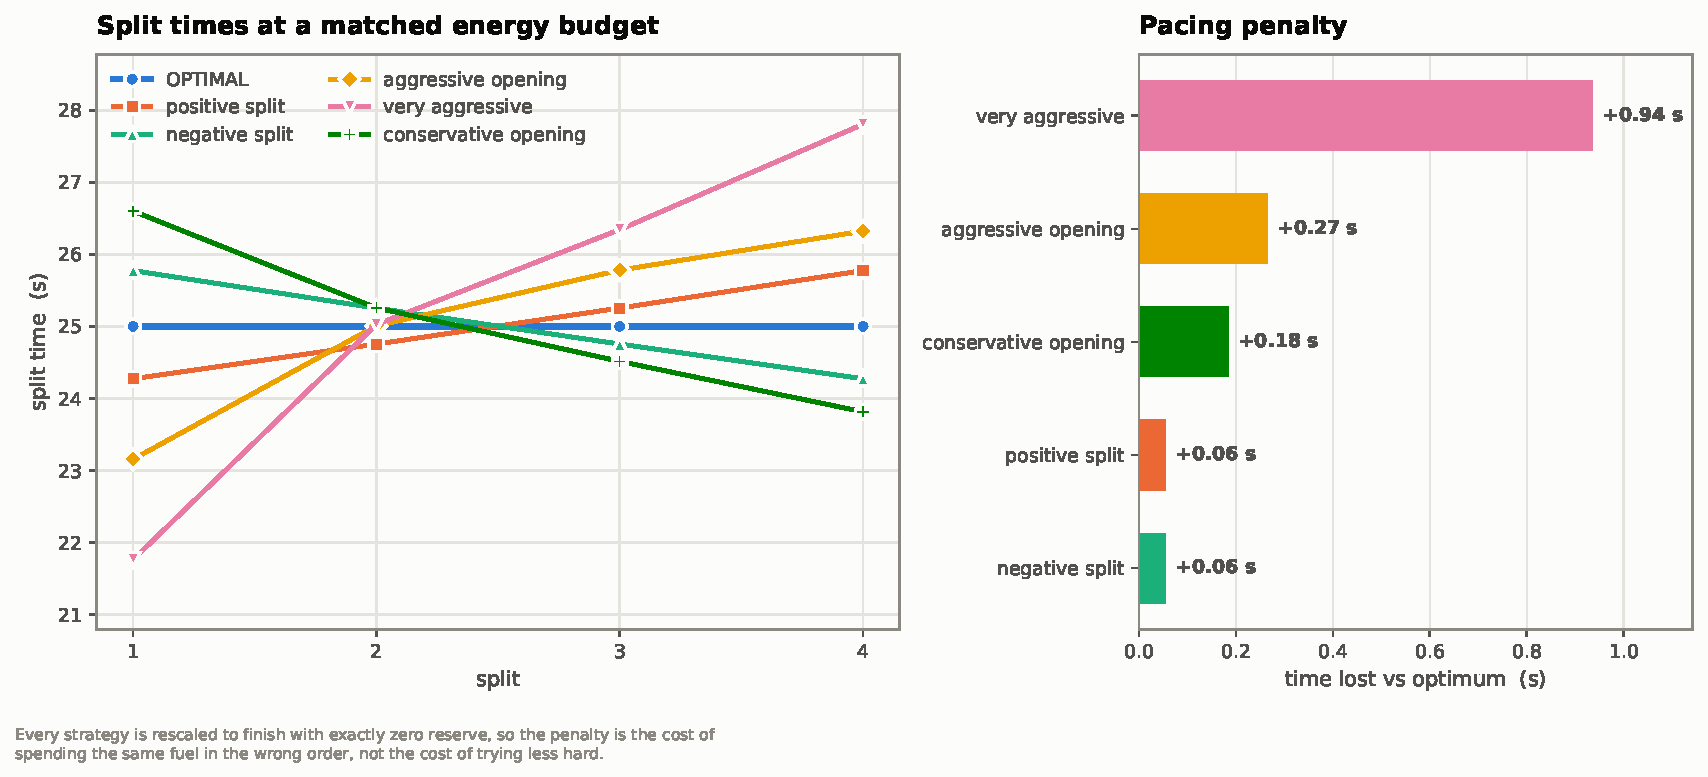
\includegraphics[width=0.74\linewidth]{fig03_strategy_comparison}
\caption{Named pacing strategies at matched energy budget. The observed
elite profile, once the dive credit is added back, lies within 0.01~s of the
even optimum.}
\label{fig:strategies}
\end{figure}

\begin{figure}[htbp]
\centering
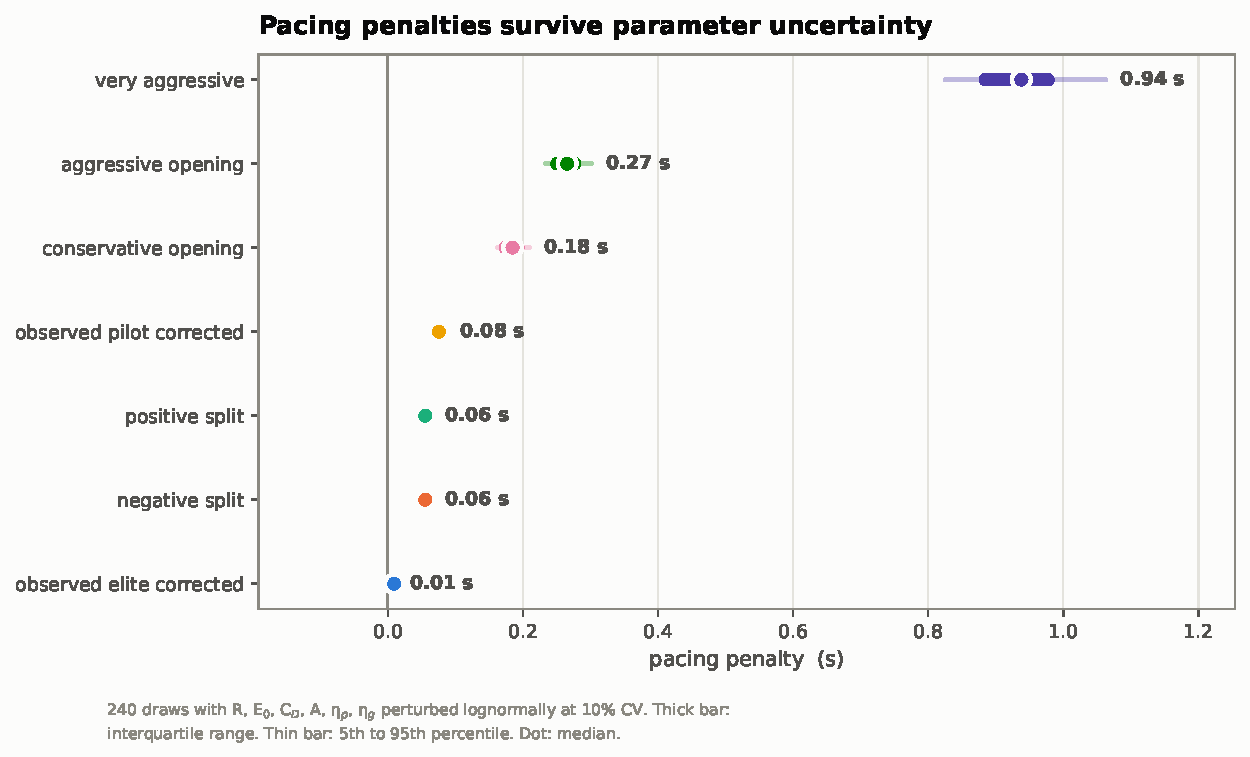
\includegraphics[width=0.7\linewidth]{fig15_penalty_robustness}
\caption{Pacing penalties under 240 seeded Monte Carlo draws of the
physiological block (10\% CV). The ordering of strategies survives every
draw; magnitudes move by about 15\%.}
\label{fig:robust}
\end{figure}

\subsection{The engine sets the speed, not the shape}

Theorem~\ref{thm:shape} says the optimal shape is independent of every
engine and hull parameter; Figure~\ref{fig:elasticity} shows how strongly
those parameters act on everything else. A 10\% change in either the drag
area $A$ or the drag coefficient $C_D$ moves the optimal race time by
7.4~s (elasticity 0.37), the same change in either efficiency moves it by
7.4~s the other way, and $R$ and $E_0$ move it by 5.3~s and 2.1~s
(elasticities 0.26 and 0.11). Not one of these changes moves the first-lap
share by more than $10^{-8}$. Only the fatigue couplings and the kinetic
time constant do anything to shape or to timing beyond the budget: stepping
$\beta_x$ from 0 to 0.05 lowers the optimal first-lap share by 0.15 points
and costs 0.91~s, while stepping $\tau$ from 0 to 2~s costs 0.53~s and
leaves the shape exactly even, as Proposition~\ref{prop:kinetics} says it
must. The archetype experiment (Figure~\ref{fig:archetypes}) makes the same
point at the level a coach would recognize: seven swimmers calibrated to the
same 1:43.0 --- aerobic-dominant, anaerobic-dominant, high-drag, low-drag
and reference --- all receive an identical, exactly even prescription
(shape spread below $10^{-8}$), and only the two fatigue archetypes differ,
the fatigue-prone swimmer ($\beta_x=0.35$) at $(.2405,.2470,.2533,.2592)$
and the fatigue-resistant one ($\beta_x=0.08$) at $(.2476,.2492,.2508,.2524)$.
The intuition that a stronger athlete has earned a faster opening lap finds
no support here; what would earn one is a \emph{smaller} fatigue coupling.

\begin{figure}[htbp]
\centering
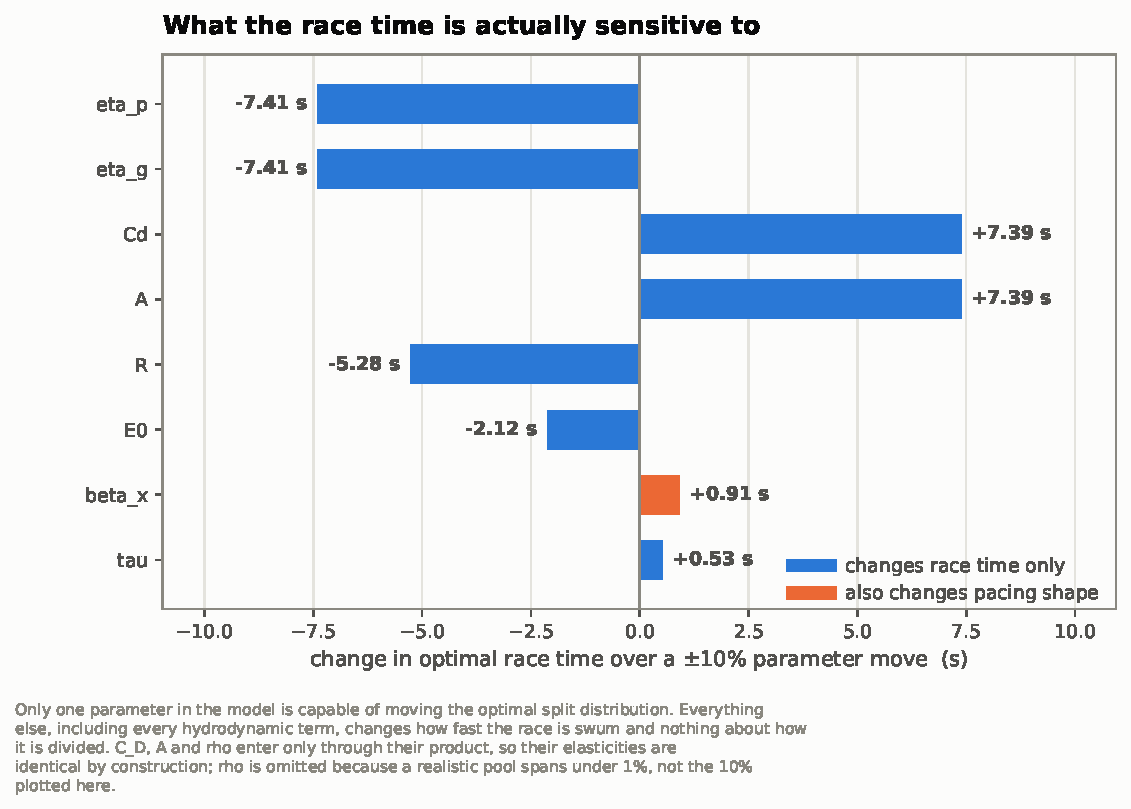
\includegraphics[width=0.7\linewidth]{fig13_elasticity}
\caption{Race-time elasticities under $\pm10\%$ parameter perturbations. The
drag and efficiency block dominates race time; none of the engine or hull
parameters moves the optimal shape.}
\label{fig:elasticity}
\end{figure}

\begin{figure}[htbp]
\centering
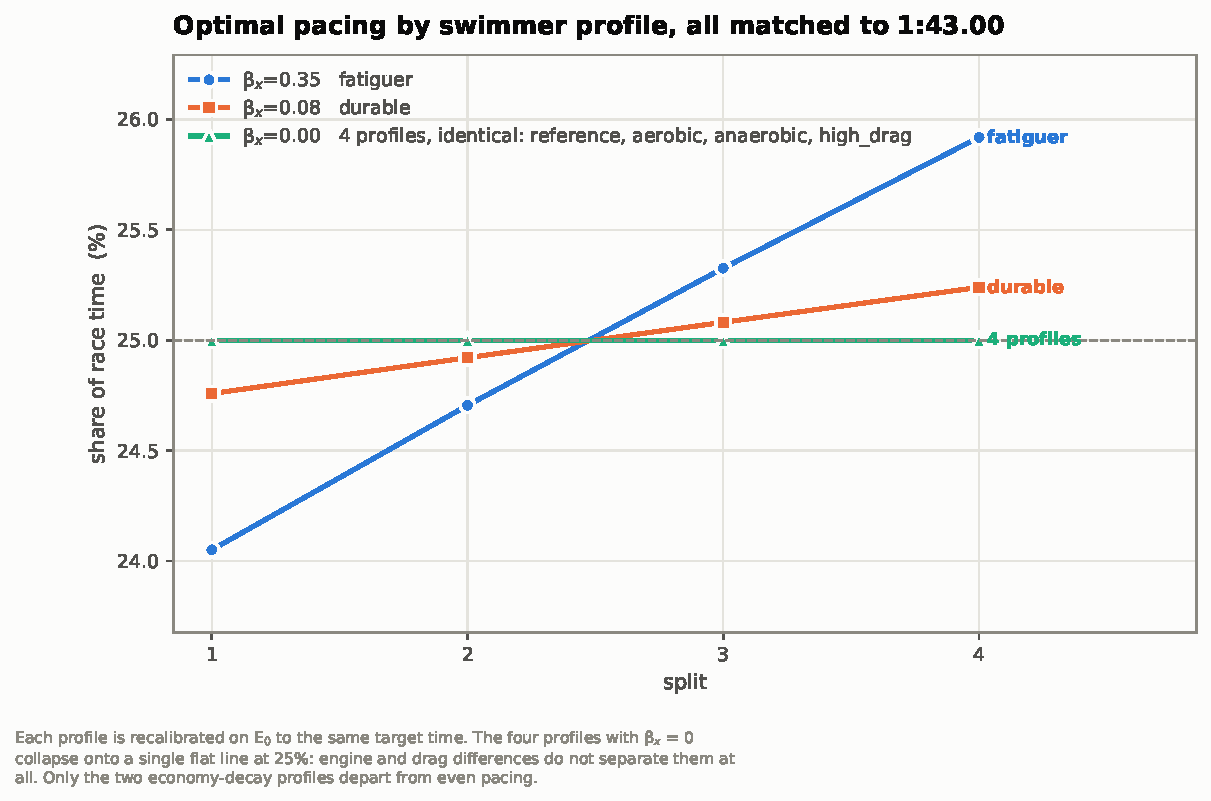
\includegraphics[width=0.74\linewidth]{fig12_archetypes}
\caption{Seven archetypes calibrated to the same target time. Only the
fatigue couplings change the prescribed shape.}
\label{fig:archetypes}
\end{figure}

\subsection{Mechanisms as shapes}

Figure~\ref{fig:mechanisms} stacks the mechanisms on the reference swimmer.
Oxygen kinetics with $\tau=20$~s costs 5.5~s and with $\tau=30$~s costs
8.4~s, in both cases with an exactly even optimum. Position-coupled decay at
$\beta_x=0.15$ and $0.30$ yields near-linear positive splits,
$(.2456,.2486,.2515,.2543)$ and $(.2417,.2474,.2528,.2581)$; reserve-coupled
decay at $\beta_E=0.30$ yields a strong negative split
$(.2815,.2605,.2382,.2198)$. The heat-map of the first-lap share over the
$(\beta_x,p)$ plane (Figure~\ref{fig:heatmap}) shows the whole M3 family at
once: the share falls monotonically in $\beta_x$ and rises toward $0.25$ as
the cost exponent $p$ grows, exactly the $w_i^{1/p}$ dependence of
Eq.~\eqref{eq:shape}. Two consequences matter for the empirical section.
First, the differences between the three shape classes are of order one to
three percentage points per lap, an order of magnitude larger than the
race-to-race scatter of shares within a class, so even a few hundred races
can separate the classes if the start is handled. Second, the differences
\emph{within} the positive class, M3 against M4, are of order a tenth of a
point per lap at the registry couplings, which is the same order as the
effect of moving the dive credit by a few tenths of a second. The theory
therefore predicts, before any data, where the empirical comparison will be
decisive and where it will be hostage to the start.

\begin{figure}[htbp]
\centering
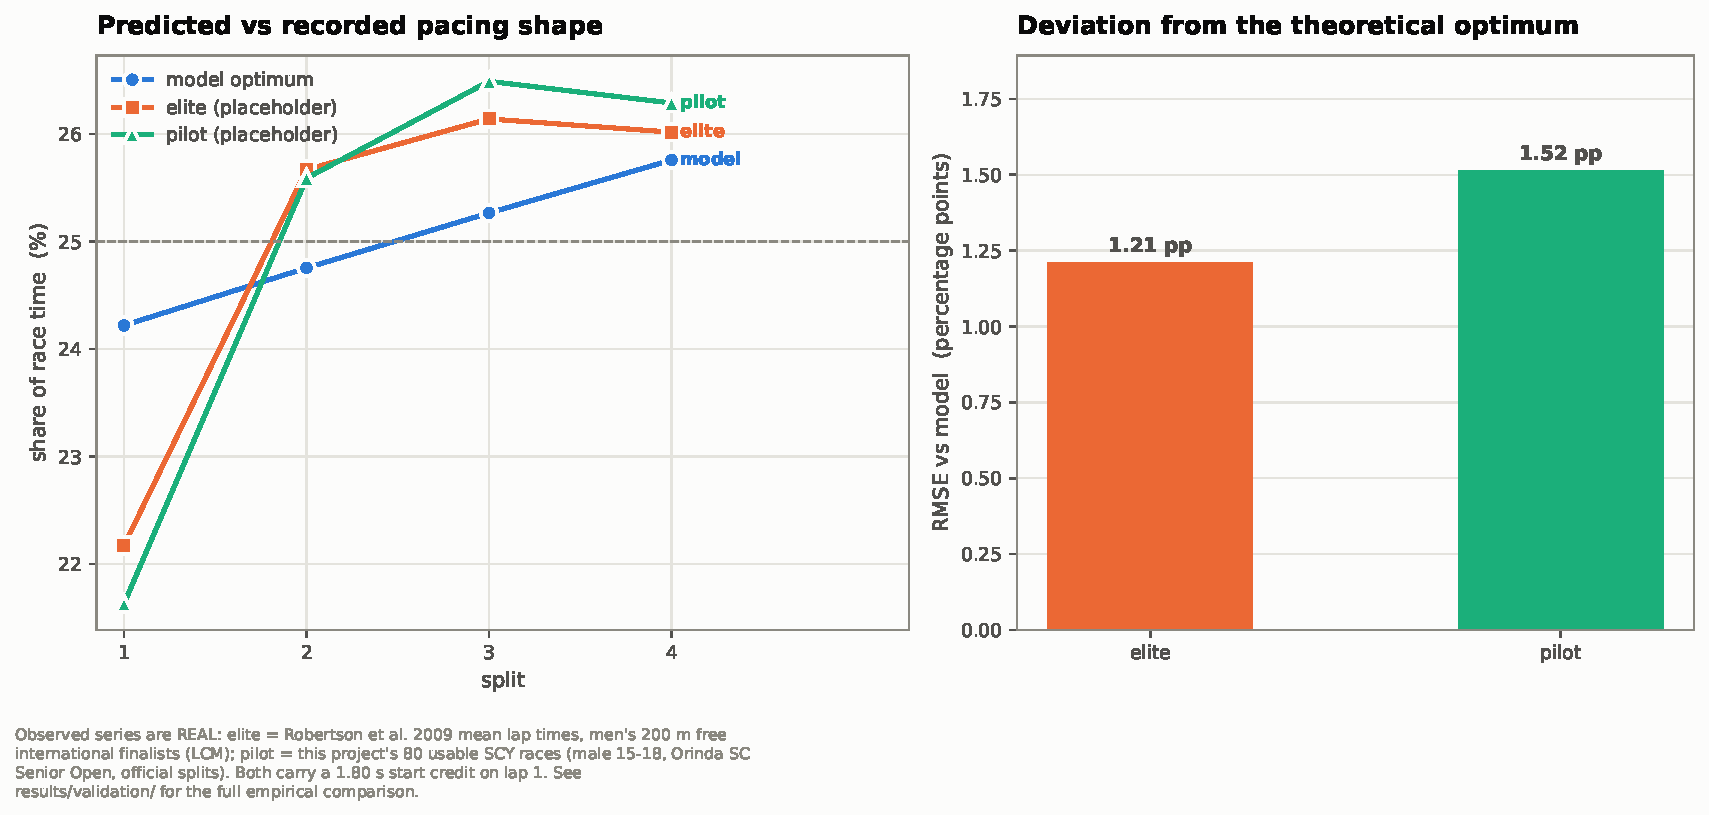
\includegraphics[width=0.74\linewidth]{fig09_theory_vs_observed}
\caption{Model optima under each mechanism against observed strategy shapes.
The mechanisms collapse onto three shape classes: even, negative, positive.}
\label{fig:mechanisms}
\end{figure}

\begin{figure}[htbp]
\centering
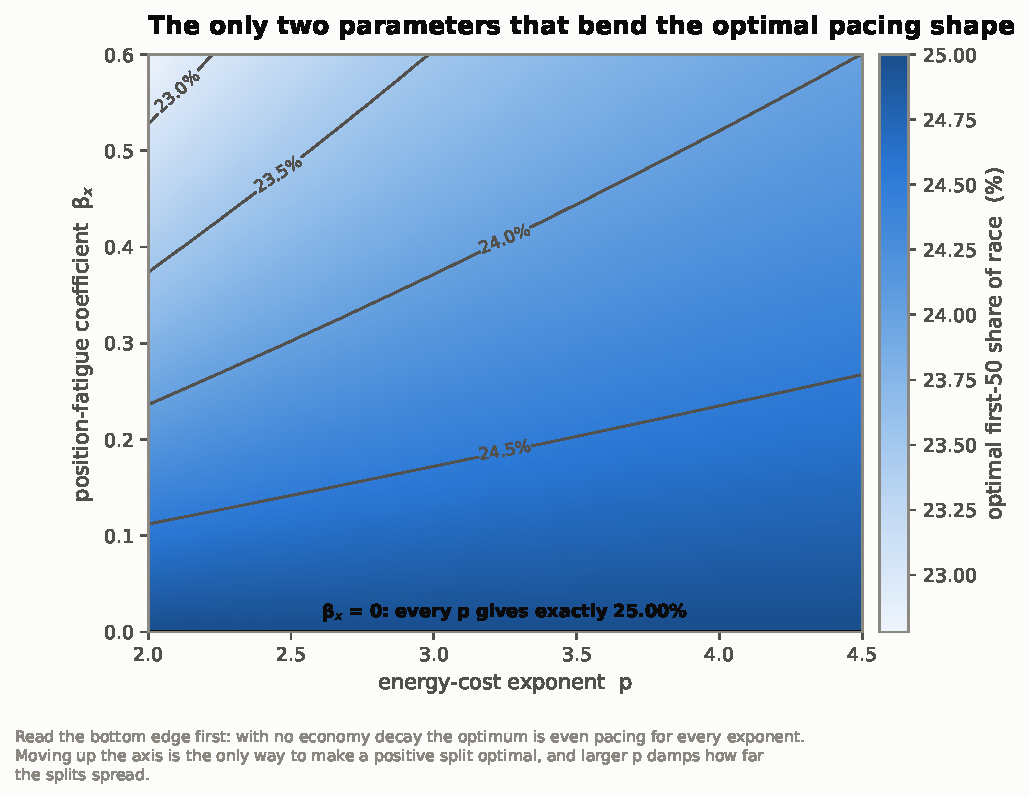
\includegraphics[width=0.55\linewidth]{fig14_shape_heatmap}
\caption{Optimal first-lap share over the position-fatigue coefficient and
the cost exponent, the only two parameters that enter the M3 shape.}
\label{fig:heatmap}
\end{figure}

\subsection{What the working swimmer prescribes}

The working swimmer used for prescriptions is the M3 variant at the registry
coupling $\beta_x=0.28$, recalibrated to 1:40.0. Its optimum is
$(.2422,.2475,.2527,.2576)$: 24.22, 24.75, 25.27, 25.76~s. Against it, even
pacing costs 0.056~s, a negative split of the same magnitude costs 0.22~s,
the conservative opening 0.43~s and the aggressive opening 0.08~s. Which
direction of error is cheaper thus depends on which mechanism is true, and
that is the question the data are asked next.

\FloatBarrier

%% Section stub: filled by its own commit per ATOMIC_COMMIT_ROADMAP.md
\section{Results Empirical}\label{sec:results-empirical}
[Pending.]

\section{Discussion}\label{sec:discussion}

\subsection{What was learned about mechanism}

The theoretical half of the paper reduced ``why do swimmers fade'' to a
sign-and-shape question, and the data answered the sign part cleanly. In
345 official races the profile is positively split, the reserve-coupled
mechanism M2 is sign-contradicted and remains the worst model even after
its coupling is fitted to the bound, and the even class is rejected on the
held-out set by a margin of 0.20 percentage points with an interval that
does not approach zero. Whatever makes late yards dearer than early ones in
a 200-yard freestyle, it is not the value of a full reserve. The positive
sign survives every credit in the registered band but the last; the
rejection of the even class holds for credits up to 2.6~s, which covers
the elite-anchored value and everything below it but not the field-pace
values above it. Within that qualification, it is the empirical result we
are most confident of.

The shape part was not answered, and the reason is instructive. M3 and M4
tie on held-out accuracy because they err in opposite directions on the
one statistic that was supposed to separate them: the observed fade is
front-loaded in kind, as M4 predicts, but only about two thirds as
front-loaded as the fitted M4 requires and far more than the fitted M3
allows. A mechanism between them --- a cost that rises with position
\emph{and} a ceiling that binds early --- would fit better, but adding it
would be a third one-parameter model chosen after the data were seen, and
we decline to do that here. The honest statement is that a single
one-parameter mechanism of either kind captures the mean profile to within
about half a percentage point per lap, that the residual is the finishing
kick, and that the fade's distribution between the early and late laps is
the next thing a model of this class must get right.

\subsection{The start credit is the problem}

The pilot showed the start-credit confound qualitatively; the registered
evaluation quantifies it. Across the literature-anchored band the fitted
$\beta_x$ moves by a factor of thirty and the held-out ranking passes
through three different winners. The fatigue mechanisms differ from each
other by tenths of a percentage point per lap; a tenth of a second of dive
credit moves the corrected first-lap share by about a tenth of a point.
This is not a statistical limitation to be cured by more races --- the
confidence intervals on the held-out RMSEs are already narrow relative to
the model differences at any fixed credit --- but a modelling limitation:
the free-swimming model is asked to explain a lap that is not free swimming,
and how much of that lap to credit to the dive is unknown to within a
second. The plan's start-uncertainty clause was written for exactly this
outcome, and we report it as the clause requires. Two remedies follow, in
order of value. First, measure the credit: 15~m split times are recorded at
some meets and published at almost none, and a single meet with them would
pin the credit for its field to a few tenths. Second, model it: a
pace-dependent term $c(v)=15/v-t_{15}$, with $t_{15}$ from the start
literature, replaces a constant that is wrong in a known direction for
slower swimmers and would remove the artefactual part of the ``faster
swimmers pace more evenly'' pattern before it is interpreted.

\subsection{The finishing kick}

Half the races in the dataset have a fourth lap faster than the third, and
the mean profile has its slowest lap third. No mechanism in the family can
produce this, and the reason is structural rather than parametric: every
cost multiplier we consider is monotone in position or reserve, and every
ceiling tightens monotonically, so the optimal lap times are monotone.
Three explanations are compatible with the data and none is tested by it.
A swimmer racing under uncertainty about their own reserve rationally holds
a margin until the finish is certain and then spends it; that is an
optimal-control problem with a stochastic state, not a deterministic one,
and it produces an end spurt. A swimmer racing a field rather than a clock
responds to the swimmers beside them, which the model excludes by design.
And a swimmer's underwater work off the last turn may simply be better,
because there is nothing to save it for. The first explanation is the most
interesting because it is a model, and it predicts something testable: the
size of the kick should fall as a swimmer's experience of the event grows
and their uncertainty about their state shrinks.

\subsection{Deviation and performance}

The pre-registered null on H1 was the expected outcome at this sample size
and it arrived. It should be read narrowly. The theory predicts that a 5\%
opening error costs 0.09~s in a 100~s race; the race-to-race noise in a
developing 16-year-old's 200 free is an order of magnitude larger, and the
expectation model available to us --- the swimmer's best earlier race in
this dataset --- is weaker still, as the three four-year-old personal bests
that manufactured a spurious curvature showed. A null under these
conditions does not say that pacing does not matter; it says that the
effect predicted by the model is below what this design can see, which the
plan said in advance. A design that could see it would use within-swimmer
comparisons across many races of one athlete, with seed times or
season-best trajectories as the expectation, and a deviation measured from
that swimmer's own fitted shape rather than the population's.

\subsection{What the theory contributes regardless}

The empirical section cannot yet say which fatigue mechanism is true, but
the structural results do not depend on it. Even pacing is the unique
optimum of every budget-constrained model with a velocity-only cost, so a
fade is always evidence of a mechanism and never a consequence of fitness;
the optimal shape is invariant to the engine and the hull, so no swimmer
has earned a faster opening lap by being stronger; and the penalty for
pacing error is quadratic and small near the optimum, so the difference
between a good pacing plan and the best one is hundredths of a second while
the difference between a good one and a bad one is tenths. The elite
profile of \citet{robertson2009analysis}, once the dive is credited, costs
0.01~s against the model's optimum; the mean profile of our first pilot
costs about 0.08~s; the ``very aggressive'' opening that coaches warn
against costs nearly a second. Which small error is cheapest depends on
the mechanism, but the ordering of large errors against small ones holds
for every mechanism considered and every parameter draw tried, and that is
the practical content of the paper.

\section{Limitations}\label{sec:limitations}

\paragraph{The start is assumed, not measured.} Every empirical statement in
this paper is conditional on the dive credit $c$. The credit is anchored to
elite 15~m start times, and the band we sweep was widened twice, by logged
amendment, once we converted those times to this field's slower pace; but
no source in our data publishes a 15~m split, so the credit is never
observed for any race we analyse. Because the credit and both positive-split
couplings push lap~1 the same way, the fitted $\beta_x$ and $\gamma$ are
credit-conditional estimates, and the width of the credit band is the width
of our ignorance about them. A pace-dependent start term,
$c(v) \approx 15/v - t_{15}$, and 15~m timing at even one meet would do more
for the model comparison than any additional race sheet.

\paragraph{Turns and underwaters are folded into $\phi$.} Short-course yards
racing contains seven turns in 200 yards, and the underwater phase is faster
than surface swimming. The model represents the whole course discount by one
calibrated factor $\phi$ and treats each 50 as free swimming at constant
velocity. The shape-invariance theorem means $\phi$ cannot move the M3
optimum, so this does not bias the shape comparison, but it does mean the
model cannot distinguish a swimmer who fades because of surface economy from
one whose turns deteriorate; both appear as $\beta_x$.

\paragraph{Constant velocity within a 50.} Cost is convex in velocity, so
this systematically understates energy cost, and the missing cost is absorbed
into the calibrated engine. It also excludes by assumption the within-lap
oscillation mechanisms of the optimal-control literature; split-level data
cannot test those in either direction.

\paragraph{One region, one course, a broad field.} All eleven meets are in
Northern California; the sample is one competitive culture and a handful of
pools. Final times span 1:37 to 2:40, a developmental range in which pacing
skill itself varies, and the population rule admits 54 races on club-linked
rather than published age. We report the published-age stratum separately
and the conclusions do not change, but a replication elsewhere, on
long-course metres, and on female and older swimmers is required before any
of this is a statement about the 200 freestyle in general.

\paragraph{Preliminary swims and the finishing kick.} Fifty-seven usable
races are preliminaries, which may be paced to qualify rather than to
minimize time. And the observed mean profile has a feature none of the five
models can produce: the third lap is the slowest and the fourth is faster
than it. Every model in the family predicts monotone lap times, because
every mechanism is monotone in position or reserve. A terminal kick is the
signature of a swimmer holding something back and spending it once the
finish is certain, which is a rational response to uncertainty about one's
own state or a tactical response to the field, and neither is in the model.

\paragraph{Fitted parameters are not physiology.} $\beta_x$, $\gamma$ and
$\beta_E$ are estimates under this model family, conditional on the start
credit, on the constant-velocity assumption and on the calibrated engine.
They are not measurements of any swimmer, and we have taken care nowhere to
describe them as such. The same applies with more force to the engine
parameters $E_0$, $R$ and $\phi$, which are calibrated to reproduce a target
time and, by Theorem~\ref{thm:shape}, are not identifiable from pacing data
at all.

\paragraph{Expectation is weak.} The pre-race personal best is derived only
from earlier rows in this dataset, so for most swimmers it is one earlier
race, often months before, in a developing athlete. Improvement on that
number mixes training gains with pacing quality, which is one reason the
deviation--performance regression was pre-registered as likely underpowered
and why its result is reported as a null rather than explained away.

\paragraph{What we did not do.} We did not fit any engine or hull parameter
to pacing data, did not use AIC or likelihood comparison, did not examine
the test set before the registered evaluation, and did not adjust anything
after it. The exploratory 80-race pilot informed the start-credit band and
exposed the sign error; both are logged as amendments made before any
calibration. We regard the ordering of those steps as the main
methodological contribution of the empirical half of the paper.

\section{Conclusion}\label{sec:conclusion}

We asked what pacing minimizes 200-yard freestyle time under realistic
energetic and fatigue constraints, and whether competitive swimmers use it.
On the first question the answer has a structure that does not depend on
parameters: under a fixed energy budget with a velocity-only cost, even
pacing is the unique optimum for every cost exponent above one, and with
position-coupled economy decay the optimal split allocation
$t_i\propto w_i^{1/p}$ is invariant to aerobic capacity, anaerobic
capacity, drag and efficiency. Fitness sets the speed of the race and not
its shape, oxygen kinetics slow the race and do not bend it, and every
departure of a real race from even pacing is evidence about a mechanism
outside the budget.

On the second question we built a verified pipeline from official result
sheets to anonymized, checksum-registered data, wrote and froze an analysis
plan before any race was in hand, and tested five fatigue mechanisms on 345
races by male swimmers aged 15--18 with a swimmer-grouped held-out set
opened once. The races are positively split; the even and negative-split
mechanisms are rejected on held-out accuracy at the elite-anchored start
credit; the two positive-split mechanisms, position-coupled cost and a
fatigue-coupled velocity ceiling, tie, because the observed fade is
front-loaded in kind but between them in degree. The ranking among the
surviving models changes inside the literature-anchored band of dive-start
credits, which under the registered plan means the data cannot distinguish
them given start uncertainty; the hypothesis that swimmers nearer the
predicted optimum perform better relative to expectation returned the null
the plan anticipated; and the mean profile carries a finishing kick that no
monotone mechanism can produce.

The next steps are set by those findings rather than by ambition. The
dive-start credit must be measured, with 15~m splits, or at least modelled
as a function of pace, before any fatigue coupling fitted to split sheets
can be interpreted. The finishing kick calls for a model with uncertainty
in the swimmer's state, which is a different and more interesting
optimization problem than the deterministic one solved here. And the
deviation--performance question needs many races of few swimmers with a
real expectation model, not few races of many swimmers with a stale one.
The code, the analysis plan with its amendment log, the dataset register
with the digests of every official source, and every number in this paper
are in the project repository, so that the next attempt can start where
this one stopped rather than where it started.


\bibliographystyle{plainnat}
\bibliography{../literature/references}

\end{document}
